\section{Examenvragen}

\subsection{Reguliere talen}

\subsubsection{Vraag 1 - GNFA}

\textit{Bewijs dat een reguliere taal beschreven door een reguliere expressie door een eindige toestandsautomaat wordt herkend. Doe dit door van de automaat een gegeneraliseerde niet-deterministische eindige toestandsautomaat te maken. Beschrijf in detail hoe uit die GNFA een reguliere expressie kan worden afgeleid.}

\paragraph{Algoritme om de omzetting uit te voeren.}
\begin{enumalgo}
  \item Generaliseer de NFA:
    \begin{itemize}
    \item Voer een nieuwe begintoestand $q_s$ in.
    \item Voer een nieuwe (unieke) eindtoestand $q_e$ in.
    \item Teken $\epsilon$-boog van $q_s$ naar de oude begintoestand.
    \item Teken $\epsilon$-boog van elke oude eindtoestand naar $q_e$.
    \item Vul de automaat aan met $\phi$-bogen waar er bogen ontbreken. (Zie definitie \ref{def:gnfa})
    \item Neem parallelle gerichte bogen samen met de unie van hun labels.
    \end{itemize}
  \item Reduceer de GNFA:
    \begin{itemize}
    \item Als $Q \setminus \{q_s, q_e\} = \emptyset$, ga naar stap 3.
    \item Voer een reductiestap uit door een willekeurige toestand $q \in Q \setminus \{q_s, q_e\}$ te verwijderen. De basis reductiestap:\\
    \begin{tabular}{>{\centering\arraybackslash}m{3.5cm}>{\centering\arraybackslash}m{1cm} >{\centering\arraybackslash}m{4cm}}
\begin{nfa}
  \node[state] (A)                     {$q_a$};
  \node[state] (X)  [below right of=A] {$q$};
  \node[state] (B)  [above right of=X] {$q_b$};
  
  \path (A) edge [bend left]  node {$E_4$} (B)
            edge [bend right] node {$E_1$} (X)
        (X) edge [loop below] node {$E_2$} (X)
            edge [bend right] node {$E_3$} (B);
  \addvmargin{1mm}
\end{nfa} & $\longrightarrow$ & \begin{nfa}
  \node[state] (A)                   {$q_a$};
  \node[state] (B)  [right=2.5cm of A] {$q_b$};
  
  \path (A) edge []  node {$E_4|E_1(E_2)^*E_3$} (B);
  \addvmargin{1mm}
\end{nfa}
\end{tabular}
    \item Herhaal stap 2.
    \end{itemize}
  \item Bepaal de reguliere expressie die af te lezen is als label op de boog tussen $q_s$ en $q_e$.
  \end{enumalgo}
  
\paragraph{Bewijs.}   We bewijzen dit door aan te tonen dat een NFA kan omgezet worden naar een reguliere expressie die dezelfde taal bepaalt. Daarom tonen we aan dat bij algoritme \ref{alg:nfagnfa} de verzameling van aanvaarde strings in elke stap niet verandert.
  
  We kunnen een pad om een string te accepteren doorheen toestanden van een GNFA beschrijven als $E_1E_2E_3...E_n$ met $n$ het aantal toestanden om de eindtoestand te bereiken en $E_i$ reguliere expressies. We verwijzen naar de GNFA voor een reductiestap met $GNFA_{voor}$ en erna met $GNFA_{na}$.
  \begin{enumalgo}
  \item De omzetting van NFA naar GNFA wijzigt de verzameling aanvaarde strings niet:
  \begin{itemize}
  \item Stel dat NFA dezelfde taal $L_E$ bepaalt als een reguliere expressie $E$. Een nieuwe begintoestand toevoegen met een $\epsilon$ boog naar de oude staat gelijk aan de expressie $\epsilon E$, dewelke gelijk is aan $E$.
  \item Stel dat NFA dezelfde taal $L_E$ bepaalt als een reguliere expressie $E$. Een nieuwe eindtoestand toevoegen met een $\epsilon$ bogen van de oude toestanden naar de nieuwe, staat gelijk aan de expressie $E\epsilon$, dewelke gelijk is aan $E$.
  \item Het toevoegen van de extra bogen om de GNFA te vervolledigen wijzigt de verzameling aanvaarde talen niet. Deze $\phi$-bogen kunnen niet gevolgd worden en dus kunnen er geen toestanden bereikt worden die voordien niet bereikt konden worden.
  \item Indien we twee parallelle gerichte bogen met labels $a_1 \in \Sigma$ en $a_2 \in \Sigma$ samennemen als een unie van die labels, dan verandert de verzameling aanvaarde strings niet. We kunnen immers de reguliere expressie $E_1|E_2$ met $E_1 = a_1$ en $E_2 = a_2$ omzetten naar een NFA met twee toestanden waarvan tussen er twee parallelle gerichte bogen lopen die de labels $a_1$ en $a_2$ hebben.
  \end{itemize}
  \item De basis reductiestap om de GNFA te reduceren wijzigt de verzameling aanvaarde strings niet. Bij het verwijderen van een willekeurige toestand $q$ zeggen we:
  \begin{itemize}
  \item Indien een string $s$ aanvaard wordt door $GNFA_{voor}$ met een pad dat $q$ niet bevat, dan wordt wordt die ook aanvaard door $GNFA_{na}$ omdat het pad ongewijzigd blijft. Als het pad $q$ wel bevat, dan zijn er twee toestanden $q_a$ en $q_b$ zodanig dat $q_aq^nq_b$ met $n > 0$ een opeenvolging is in dat pad. De reguliere expressies op de bogen $q_aq$, $qq$ en $qq_b$ zijn dan $E_1$, $E_2$ en $E_3$ respectievelijk en bijgevolg is dat deel van het pad gelijk aan de expressie $E_1(E_2)^*E_3$. Die expressie vinden we terug op de boog $q_aq_b$ in $GNFA_{na}$, dus wordt dezelfde string ook aanvaard door $GNFA_{na}$.
  \item Als een string $s$ aanvaard wordt door $GNFA_{na}$, kan het pad door $GNFA_{na}$ de toestand $q$ uiteraard niet bevatten. Op een boog $q_aq_b$ staat de reguliere expressie $E_4|E_1(E_2)^*E_3$, wat wil zeggen dat de string moet voldoen aan aan de expressie $E_4$ of de expressie $E_1(E_2)^*E_3$. In $GNFA_{voor}$ komt dat overeen met het bereiken van $q_b$ uit $q_a$ door een boog $q_aq_b$ te volgen met expressie $E_4$, ofwel bogen $q_aq^nq_b$ met $n > 0$ waar de toestand $q$ \'e\'en of meerdere keren voorkomt. De reguliere expressies op de bogen $q_aq$, $qq$ en $qq_b$ zijn dan $E_1$, $E_2$ en $E_3$ respectievelijk. De string wordt door $GNFA_{voor}$ dus ook aanvaard wanneer $q$ wel of niet op het pad door $GNFA_{voor}$ ligt.
  \end{itemize}
  \end{enumalgo}

\subsubsection{Vraag 1 (Bijvraag 1)}

\textit{Kan voor een PDA ongeveer hetzelfde gedaan worden door een gegeneraliseerde PDA op te stellen?}

Nee, want een GPDA formaat bestaat niet. Bij het construeren van een PDA uit een CFG, bekomen we een PDA met drie toestanden. Zo'n PDA kunnen we makkelijk naar een CFG converteren, maar niet elke PDA heeft drie toestanden en er is geen gelijkaardige manier zoals bij een GNFA om de PDA te reduceren.

\subsubsection{Vraag 1 (Bijvraag 2)}

\begin{center}
\renewcommand{\arraystretch}{1.5}
\begin{tabular}{>{\centering\arraybackslash}m{5cm}>{\centering\arraybackslash}m{1cm} >{\centering\arraybackslash}m{5cm}}
\begin{nfa}
  \node[state] (A)                     {$A$};
  \node[state] (X)  [below right of=A] {$X$};
  \node[state] (B)  [above right of=X] {$B$};
  
  \path (A) edge [bend left]  node {$E_4$} (B)
            edge [bend right] node {$E_1$} (X)
        (X) edge [loop below] node {$E_2$} (X)
            edge [bend right] node {$E_3$} (B);
  \addvmargin{1mm}
\end{nfa} & $\longrightarrow$ & \begin{nfa}
  \node[state] (A)                   {$A$};
  \node[state] (B)  [right=3cm of A] {$B$};
  
  \path (A) edge []  node {$E_4|E_1(E_2)^*E_3$} (B);
  \addvmargin{1mm}
\end{nfa}
\end{tabular}
\end{center}

\textit{Stel dat het linkse deel toestand B niet bevat, de boog met $E_3$ van $X$ naar $A$ gaat en de boog met $E_4$ van $A$ naar zichzelf gaat. Kan dit omgevormd worden op methode gelijkaardig aan die beschreven is in de cursus?}

\begin{center}
\begin{nfa}
  \node[state] (A)              {$A$};
  \node[state] (X) [right of=A] {$X$};
  
  \path (A) edge [bend left]  node {$E_1$} (X)
            edge [loop left]  node {$E_4$} (A)
        (X) edge [bend left]  node {$E_3$} (A)
            edge [loop right] node {$E_2$} (X);
  \addvmargin{1mm}
\end{nfa}
\end{center}

Ja, we elimineren eerst het pad van $X$ naar $A$. We voeren een nieuwe toestand $Y$ in en gebruiken de standaard eleminatie om het pad van $Y$ naar $X$ door $A$ te behandelen:

\begin{center}
\renewcommand{\arraystretch}{1.5}
\begin{tabular}{>{\centering\arraybackslash}m{5cm}>{\centering\arraybackslash}m{1cm} >{\centering\arraybackslash}m{5cm}}
\begin{nfa}
  \node[state] (A)                   {$A$};
  \node[state] (X) [above right=.25cm and 2cm of A] {$X$};
  \node[state] (Y) [below right=.25cm and 2cm of A] {$Y$};
  
  \path (A) edge [bend left]  node {$E_1$}      (X)
            edge [loop left]  node {$E_4$}      (A)
        (X) edge [bend left]  node {$\epsilon$} (Y)
            edge [loop right] node {$E_2$}      (X)
        (Y) edge [bend left]  node {$E_3$}      (A)
            edge [bend left]  node {$\epsilon$} (X);
  \addvmargin{1mm}
\end{nfa} & $\longrightarrow$ & \begin{nfa}
  \node[state] (X) []                {$X$};
  \node[state] (Y) [below=.75cm of X] {$Y$};
  
  \path (X) edge [bend left]  node {$\epsilon$}               (Y)
            edge [loop right] node {$E_2$}                    (X)
        (Y) edge [bend left]  node {$\epsilon|E_3(E_4)^*E_1$} (X);
  \addvmargin{1mm}
\end{nfa}
\end{tabular}
\end{center}

Nu we de boog van $X$ naar $A$ ge\"elemineerd hebben, kunnen we de resterende bewerkingen uitvoeren om de lussen van de knopen op de boog tussen $A$ en $X$ te plaatsen:

\begin{center}
\renewcommand{\arraystretch}{1.5}
\begin{tabular}{>{\centering\arraybackslash}m{4cm}>{\centering\arraybackslash}m{1cm} >{\centering\arraybackslash}m{5.5cm}}
\begin{nfa}
  \node[state] (A)              {$A$};
  \node[state] (X) [right of=A] {$X$};
  
  \path (A) edge []           node {$E_1$} (X)
            edge [loop left]  node {$E_4$} (A)
        (X) edge [loop above] node {$E_2|E_3(E_4)^*E_1$} (X);
  \addvmargin{1mm}
\end{nfa} & $\longrightarrow$ & \begin{nfa}
  \node[state] (A)              {$A$};
  \node[state] (X) [right=4cm of A] {$X$};
  
  \path (A) edge [] node {$(E_4)^*E_1(E_2|E_3(E_4)^*E_1)^*$} (X);
  \addvmargin{1mm}
\end{nfa}
\end{tabular}
\end{center}

\subsubsection{Vraag 2 - NFA naar DFA}

\textit{Beschrijf in detail de transformatie van een niet-deterministische eindige toestandsautomaat naar een equivalente deterministische eindige toestandsautomaat.}

  We construeren een DFA ($Q_d$, $\Sigma$, $\delta_d$, $q_{sd}$, $F_d$) uit een NFA ($Q_n$, $\Sigma$, $\delta_n$, $q_{sn}$, $F_n$) zodanig dat $L_{NFA} = L_{DFA}$ als volgt:
  \begin{itemize}
  \item $Q_d = \powerset(Q_n)$: Elke toestand van de DFA is een verzameling van toestanden van de NFA. Onbereikbare toestanden zullen we later verwijderen, waardoor zal gelden: $Q_d \subseteq \powerset(Q_n)$.
  \item \bm{$\delta_d: (\powerset(Q_n) \times \Sigma) \rightarrow \powerset(Q_n)$}\\$\delta_d(\dfastate, a) = eb(\delta_n(\dfastate, a))$ voor $\dfastate \in Q_d$: Voor een symbool $a$ is er vanuit de toestand van de DFA $\dfastate$ een overgang naar de toestand van de DFA die alle toestanden van de NFA bevat die epsilon-bereikbaar zijn vanuit alle $q \in \dfastate$.
  \item $q_{sd} = eb(q_{sn})$: De starttoestand is de verzameling van toestanden van de NFA die epsilon-bereikbaar zijn vanuit de starttoestand van de NFA.
  \item $F_d = \{S|S \in Q_d, S \cap F_n \neq \emptyset\}$: Een eindtoestand van een DFA bevat altijd een eindtoestand van de NFA.
  \end{itemize}
  Om de constructie uit te voeren hebben we de volgende definities ingevoerd:
  \begin{itemize}
  \item \bm{$eb: Q_n \rightarrow \powerset(Q_n)$}\\ $eb(q) = \{x|x \in \{q\} \cup \delta_n(q, \epsilon)\}$ met $q \in Q_n$: De afbeelding die een toestand $q \in Q_n$ afbeeldt op alle epsilon-bereikbare toestanden. Een toestand $q_{next}$ is epsilon-bereikbaar uit $q$ indien $q_{next} = q$ of er een overgang bestaat zodanig dat $\delta_n(q, \epsilon) = q_{next}$.
  \item \bm{$eb: Q_d \rightarrow \powerset(Q_n)$}\\ $eb(\dfastate) = \{x|x \in \bigcup_{q \in \dfastate}eb(q)\}$ met $\dfastate \in Q_d$: De afbeelding die een toestand $\dfastate \in Q_d$ afbeeldt op alle toestanden die epsilon-bereikbaar zijn vanuit alle toestanden in $\dfastate$.
  \item \bm{$\delta_n: Q_d \times \Sigma \rightarrow \powerset(Q_n)$}\\ $\delta_n(\dfastate, a) = \{x|x \in \bigcup_{q \in \dfastate}\delta_n(q, a)\}$ met $\dfastate \in Q_d$ en $a \in \Sigma$: De afbeelding die een toestand $\dfastate \in Q_d$ afbeeldt op de verzameling van alle toestanden die voor een gegeven symbool bereikbaar zijn vanuit elke toestand in $\dfastate$.
  \end{itemize}

\textit{Beschrijf de notie van ``equivalentie van automaten'' in deze context en argumenteer waarom de transformatie ``correct'' is.}

Een NFA en DFA zijn equivalent indien ze dezelfde taal bepalen. De transformatie van een NFA naar een DFA is correct omdat de resulterende DFA de uitvoering van de NFA simuleert. Bij het uitvoeren van een DFA voor een gegeven string kunnen we telkens maar in \'e\'en toestand belanden, bij een NFA is dat niet het geval. De transformatie die we toepassen stelt ons in staat om voor elk symbool van een string te bepalen in welke toestand of combinatie van toestanden een NFA zich zal bevinden. Indien \'e\'en van die toestanden een eindtoestand is, kan de NFA de string op dat punt ook accepteren. Die constructie zelf is een DFA, omdat we nu voor elk pad door de automaat een deterministisch pad naar combinaties van toestanden hebben bepaald.

\textit{Bespreek de uitspraak ``deze transformatie is [niet] deterministisch''. (kies zelf of je die ``niet'' wil houden of niet)}

De transformatie is deterministisch omdat de resulterende DFA altijd hetzelfde is voor een bepaalde NFA.

\subsubsection{Vraag 2 (Bijvraag 1)}

\textit{Kan er zo'n DFA bestaan met minder toestanden dan de NFA?}

Het is mogelijk dat een DFA die geconstrueerd wordt uit een NFA minder toestanden heeft. Dat is mogelijk omdat verschillende toestanden van de NFA worden samengenomen en indien de onbereikbare toestanden niet in de resulterende DFA worden opgenomen, is er daarom een mogelijkheid om een kleine DFA te bekomen.

Een (triviaal) voorbeeld is bijvoorbeeld een nieuwe begintoestand introduceren in een NFA die met een $\epsilon$-boog naar de oude toestand gaat. Indien de originele NFA naar een DFA transformeert met een gelijk aantal toestanden, zal de nieuwe NFA naar een DFA transformeren die \'e\'en toestand minder heeft omdat de $\epsilon$-bereikbare toestanden samen worden genomen.


\subsubsection{Vraag 2 (Bijvraag 2)}

\textit{Werkt deze transformatie ook om van een NPDA naar een DPDA te gaan?}

Nee, het is mogelijk om voor elke CFG een PDA te construeren, maar het is niet mogelijk om een PDA om te zetten naar een deterministische PDA indien de CFL ambigu is. Dat wil zeggen dat er voor een string uit die taal meer dan \'e\'en meest-linkse afleiding bestaat. We kunnen dus geen algemeen algoritme opstellen dat een PDA omzet naar een deterministische versie van die PDA.

\subsubsection{Vraag 3 - DFA naar DFA$_{min}$}

\textit{Beschrijf in detail de transformatie van een deterministische eindige toestandsautomaat naar een equivalente deterministische eindige toestandsautomaat met een minimaal aantal toestanden.}

\paragraph{Algoritme om de overgangsfunctie van een DFA totaal te maken.}
  Indien de parti\"ele DFA niet reeds een complete DFA is, construeren we een equivalente complete DFA als volgt:
  \begin{enumalgo}
  \item We bepalen een nieuwe verzameling toestanden $Q' = Q \cup \{q_t\}$, met een nieuwe toestand $q_t$.
  \item We bepalen een nieuwe overgangsfunctie $\delta'$ voor $Q' = Q \cup \{q_t\}$ waarvoor geldt
  \begin{equation*}
  \forall q \in Q', a \in \Sigma: \delta'(q, a) = \begin{cases}
    \delta(q, a), & \text{als}\ \delta(q, a) \neq \phi\\
    q_t & \text{anders}
  \end{cases}
  \end{equation*}
  \end{enumalgo}

\paragraph{Algoritme om f-gelijke toestanden te bepalen.}
  We stellen een graaf V op met als knopen de toestanden van een gegeven DFA. We duiden een boog in $V$ tussen twee knopen $q_1$ en $q_2$ aan als $(q_1,q_2) \in V$.
  \begin{enumalgo}
  \item We voegen aan de graaf V een boog toe tussen elk paar knopen waarvan er precies \'e\'en in $F$ zit.
  \item Indien er een paar knopen $p$ en $q$ bestaat, zodanig dat $(p,q) \notin V$ en $\exists a \in \Sigma: (\delta(p, a),\delta(q, a)) \in V$, dan:
  \begin{itemize}
  \item Voeg een boog $(p,q)$ toe aan $V$.
  \item Herhaal stap 2.
  \end{itemize}
  Anders, ga naar stap 3.
  \item Stel de complementsgraaf $G$ van $V$ op. De toestanden van elk component van $G$ zijn onderling f-gelijk. De toestanden van twee verschillende componenten van $G$ zijn f-verschillend van elkaar.
  \end{enumalgo}

\paragraph{Algoritme om DFA$_{min}$ te bepalen.}
\begin{enumalgo}
  \item Verwijder alle toestanden van waaruit het niet mogelijk is om een eindtoestand $q \in F$ te bereiken en alle toestanden die niet bereikbaar zijn.
  \item Transformeer (indien nodig) de DFA naar een volledige DFA met bovenstaand algoritme.
  \item Bepaal de f-gelijke toestanden van de DFA met bovenstaand algoritme.
  \item Neem alle onderling f-gelijke toestanden samen in een enkele toestand, zodanig dat alle uitgaande bogen van alle f-gelijke toestanden nu uit hun gecombineerde toestand vertrekken en alle bogen die toekwamen in de f-gelijke toestanden nu toekomen in hun gecombineerde toestand.
  \item Verwijder (indien toegevoegd in stap 2) de toestand $q_t$, vanuit deze toestand is het niet mogelijk om de eindtoestand te bereiken.
  \end{enumalgo}
  De resulterende DFA is een minimale DFA.

\textit{Beschrijf de notie van ``equivalentie van automaten'' in deze context en argumenteer waarom er geen kleinere equivalente deterministische eindige toestandsautomaat bestaat.}

Twee automaten zijn equivalent indien ze dezelfde taal bepalen. Als twee DFA's $DFA_1$ en $DFA_2$ dezelfde taal bepalen (equivalent zijn), dan zijn hun minimale DFA's isomorf. Dat wil zeggen dat enkel de namen van hun toestanden mogen verschillen.

\textbf{Bewijs dat een minimale DFA het minimum aantal toestanden heeft.}   Stel $DFA_1$ ($Q_1$, $\Sigma$, $\delta_1$, $q_s$, $F_1$) met $Q_1 = \{q_s,q_1,q_2,...,q_n\}$ is een machine zonder onbereikbare toestanden waarvan elk paar toestanden f-verschillend zijn. Stel dat $DFA_2$ ($Q_2$, $\Sigma$, $\delta_2$, $q_s$, $F_2$) een DFA is met minder toestanden dan $DFA_1$.

  \begin{itemize}
  \item Elke toestand in $DFA_1$ is bereikbaar, dus er bestaan strings $s_i$ met $i=1...n$ zodanig dat $\delta^*_1(q_s,s_i)=q_i$.
  \item $DFA_2$ heeft minder toestanden dan $DFA_1$, dus er is een $i$ en $j$ met $i \neq j$, zodanig dat er strings $s_i$ en $s_j$ zijn waarvoor $DFA_2$ meerdere keren in dezelfde toestand komen, dus $\delta^*_2(q_s,s_i)=\delta^*_2(q_s,s_j)$.
  \item $q_i$ en $q_j$ zijn f-verschillend, dus er bestaat een string $v$ zodanig dat $\delta^*_1(q_i,v) \in F_1 \en \delta^*_1(q_j,v) \notin F_1$ of omgekeerd. Bij gevolg geldt ook $\delta^*_1(q_s,s_iv) \in F_1 \en \delta^*_1(q_s,q_jv) \notin F_1$ of omgekeerd. We zeggen dat $DFA_1$ van $s_iv$ en $s_jv$ just \'e\'en string accepteert.
  \end{itemize}
  
  We kunnen nu aantonen dat $\delta^*_2(q_s,s_iv) = \delta^*_2(\delta^*_2(q_i),v) = \delta^*_2(\delta^*_2(q_j),v) = \delta^*_2(q_s,s_jv)$, wat betekent dat $DFA_1$ en $DFA_2$ niet dezelfde taal kunnen bepalen.

\subsubsection{Vraag 3 (Bijvraag 1)}

\textit{Kan een kleinere equivalente niet-deterministische eindige toestandsautomaat (NFA) bestaan?}

Er kan een NFA bestaan die minder toestanden heeft dan een minimale DFA en nog steeds dezelfde taal bepaalt. Dit is het gevolg van de beperkingen die bij een DFA worden opgelegd, die niet gelden voor een NFA, zoals het verbod op $\epsilon$-bogen en dat er voor een bepaald symbool hoogstens \'e\'en boog uit een toestand mag vertrekken. Daarom zal een DFA (zelfs een minimale DFA) die equivalent is met een NFA, vaak meer toestanden hebben.

Een voorbeeld van een taal waarvoor dat geld is de taal bepaald door de reguliere expressie $(a|b)^*a(a|b)(a|b)$. Deze taal kan bepaald worden door een NFA met vier toestanden. De equivalente minimale DFA die dezelfde taal bepaalt heeft acht toestanden.

\subsubsection{Vraag 4 - $MN(L)$-relaties}

\textit{Geef de definitie van een Myhill-Nerode relatie over een taal $L$, of zoals we noteren een $MN(L)$-relatie.}

Een Myhill-Nerode relatie voor een taal $L$ ($MN(L)$-relatie) is een equivalentierelatie $\sim_X$ die voldoet aan de volgende eigenschappen:
  \begin{itemize}
  \item $\sim_X$ is rechts congruent\\$\forall x, y \in \Sigma^*, a \in \Sigma: x \sim_X y \Rightarrow xa \sim_X ya$
  \item $\sim_X$ verfijnt $\sim_L$\\$x \sim_X y \Rightarrow x \sim_L y$
  \item $\sim_X$ heeft een eindige index\\Het aantal equivalentieklassen van $\sim_X$ is eindig.
  \end{itemize}

\textit{Bewijs vervolgens dat een $MN(L)$-relatie bestaat als en slechts als $L$ regulier is.}

  Het bewijs wordt geleverd door aan te tonen dat het mogelijk is om een $MN(L)$-relatie te construeren uit een DFA en een DFA uit een $MN(L)$-relatie.
  \begin{itemize}
  \item Voor een gegeven DFA $D$ kan men een equivalentierelatie $\sim_D$ construeren waarvoor geldt
  \begin{equation*}
  \forall x, y \in \Sigma^*: x \sim_D y \Leftrightarrow \delta^*(q_s, x) = \delta^*(q_s, y)
  \end{equation*}
  \begin{itemize}
  \item $\sim_D$ is rechts congruent omdat geldt
  \begin{equation*}
  \forall x, y \in \Sigma^*, a \in \Sigma: xa \sim_D ya \Leftrightarrow \delta(\delta^*(q_s, x), a) = \delta(\delta^*(q_s, y), a)
  \end{equation*}
  \item $\sim_D$ verfijnt $\sim_{L_D}$, omdat $\sim_D$ een equivalentieklasse genereert voor alle strings die aanvaard worden door per eindtoestand. Bovendien is $\delta$ een totale functie en zullen alle strings die niet aanvaard worden samen in een equivalentieklasse komen. De verzameling van die equivalentieklassen is een partitie van $\Sigma^*$ die $\sim_{L_D}$ verfijnt.
  \item $\sim_D$ heeft een eindige index omdat het aantal toestanden in $D$ eindig is.
  \end{itemize}
  \item Voor een $MN(L)$-relatie kan men een DFA ($Q$, $\Sigma$, $\delta$, $q_s$, $F$) construeren die $L$ bepaalt, waarvoor geldt
  \begin{itemize}
  \item $Q = \{x_\sim|x \in \Sigma^*\}$\\
  De toestanden van de DFA zijn gelijk aan de equivalentieklassen van de $MN(L)$-relatie, dat aantal equivalentieklassen is eindig.
  \item $\delta(x_\sim, a) = (xa)_\sim$\\
  Volgt uit de rechtse congruentie eigenschap van de equivalentierelatie.
  \item $q_s = \epsilon_\sim$
  Een starttoestand wordt bereikt met $\epsilon$.
  \item $F = \{x_\sim|x \in L\}$\\
  Een eindtoestand wordt bereikt door elke string in $L$. Het aantal eindtoestanden is eindig omdat $F \subseteq Q$.
  \end{itemize}
  Tenslotte bewijzen we met inductie voor een willekeurige string $x \in \Sigma^*$ dat geldt
  \begin{equation*}
  \forall x \in \Sigma^*: x \in L_{DFA} \triangleq \delta^*(\epsilon_\sim,x) \in F \Leftrightarrow x \in L \triangleq x_\sim \in F
  \end{equation*}
  \begin{itemize}
  \item Voor een string $x$ met een lengte $l = 0$:
  \begin{equation*}
  \delta^*(\epsilon_\sim,\epsilon) = \delta(\epsilon_\sim,\epsilon) = \epsilon_\sim \Leftrightarrow x_\sim \in F
  \end{equation*}
  \item Stel dat de bewering geldt voor een string met willekeurige lengte $l$, dan geldt ze ook voor $xa$ met $a \in \Sigma$:
  \begin{equation*}
  \delta^*(\epsilon_\sim,xa) = \delta(x_\sim,a) = (xa)_\sim \Leftrightarrow x_\sim \in F
  \end{equation*}
  \end{itemize}
  \end{itemize}

\textit{Bestaat er voor een taal $L$ soms meer dan één $MN(L)$-relatie?}

Een taal $L$ waarvoor een $MN(L)$-relatie bestaat moet regulier zijn. Een mogelijke $MN(L)$-relatie voor een reguliere taal is $\sim_{DFA}$. Die equivalentierelatie wordt bepaald door alle strings die vanuit de begintoestand van de $DFA$ een willekeurige toestand bereiken te groeperen per toestand.
\begin{equation*}
\forall x, y \in \Sigma^*: x \sim_{DFA} y \Leftrightarrow \delta^*(q, x) = \delta^*(q, y)
\end{equation*}
We kunnen voor de taal $L$ een equivalente DFA opstellen die dezelfde taal bepaalt, maar niet isomorf is. De equivalentierelatie $\sim_{DFA}$ voor die DFA zal $\Sigma^*$ anders partitioneren. Bijgevolg bestaat er meer dan \'e\'en $MN(L)$-relatie voor een taal $L$.

\subsubsection{Vraag 4 - Pompend lemma}

\textit{Geef een precieze formulering van het pompend lemma voor reguliere talen en een bewijs ervan.}

Voor een reguliere taal $L$ bestaat een pomplengte $d$ zodanig dat als $s \in L$ en $|s| \geq d$, er minstens \'e\'en verdeling bestaat van $s$ in stukken $x$, $y$ en $z$ met $s = xyz$ en
  \begin{enumerate}
  \item $\forall i \geq 0: xy^iz \in L$
  \item $|y| > 0$
  \item $|xy| \leq d$
  \end{enumerate}

\paragraph{Bewijs.} Voor een DFA die een taal $L$ bepaalt nemen we een pomplengte $d = \#Q + 1$ en een willekeurige string $s = a_1a_2a_3...a_n$ met $n \geq d$. De accepterende sequentie van toestanden ($q_s = q_1$, $q_2$, ..., $q_f$) voor s heeft een lengte strikt groter dan het aantal toestanden in $Q$, dus er zijn bij de eerste $d$ toestanden zeker twee toestanden gelijk omdat er maar $d-1$ toestanden zijn. Stel dat $q_i$ en $q_j$ gelijk zijn met $i < j \leq d$, dan nemen we
  \begin{equation*}
  \begin{cases}
  x = a_1a_2...a_i\\
  y = a_{i+1}a_{i+2}...a_j\\
  z = a_{j+1}a_{j+2}...a_n
  \end{cases}
  \end{equation*}
  \begin{itemize}
  \item Eigenschap 1 geldt omdat $y$ een lus volgt en die $k$ keer herhaald kan worden voor $xy^kz \in L$.
  \item Eigenschap 2 geldt omdat $i$ strikt kleiner is dan $j$, dus bevat $y$ minstens \'e\'en element.
  \item Eigenschap 3 geldt omdat $i < j \leq d$, dus we hebben $xy$ kleiner dan (of gelijk aan) $d$ gekozen.
  \end{itemize}

\textit{Geef voorbeelden waarbij je laat zien hoe je dat lemma gebruikt om te bewijzen dat een gegeven taal regulier is en om te bewijzen dat een gegeven taal niet regulier is.}

Het pompend lemma kan niet gebruikt worden om te bewijzen dat een taal regulier is, omdat het een eigenschap definieert die elke reguliere taal heeft, maar het is niet uitgesloten dat een niet-reguliere taal die eigenschap niet heeft (en er zijn effectief niet-reguliere talen waarvan men strings kan pompen). Dus het is enkel mogelijk om aan te tonen dat een taal niet regulier is indien die een string bevat die men niet kan pompen.

We tonen aan dat een taal $L = \{a^nb^n|n \in \nat\}$ over $\Sigma = \{a,b\}$ niet regulier is.

Stel dat er voor $L$ een pomplengte $d$ bestaat, dan beschouwen we de string $s=a^db^d$. We nemen een willekeurige opdeling van $s=xyz$ met $|y| > 0$. Er zijn drie mogelijkheden:

\begin{itemize}
\item $y$ bevat enkel $a$'s: $xyyz$ bevat dan meer $a$'s dan $b$'s, dus $xyyz \notin L$ of $xz$ bevat dan meer $b$'s dan $a$'s, dus $xz \notin L$
\item $y$ bevat enkel $b$'s: $xyyz$ bevat dan meer $b$'s dan $a$'s, dus $xyyz \notin L$ of $xz$ bevat dan meer $a$'s dan $b$'s, dus $xz \notin L$
\item $y$ is van de vorm $a^ib^j$ met $i,b \in \nat_0$: $xyyz \notin L$ want het aantal $a$'s en $b$'s blijft enkel gelijk indien $i=j$ en zelfs dan wordt de volgorde niet meer gerespecteerd, er zullen $a$'s en $b$'s door elkaar staan.
\end{itemize}

\subsubsection{Vraag 4 (Bijvraag 1)}

\textit{Is er een verband tussen de kleinste DFA voor een taal en de kortste pomplengte?}

Ja, de kortste pomplengte moet steeds \'e\'en groter zijn dan het aantal toestanden in de minimale DFA. Indien dat niet het geval zou zijn, is het pompend lemma niet meer geldig voor strings die een lengte hebben gelijk aan het aantal toestanden (of voor een lengte kleiner dan dat). Intu\"itief voelen we dit aan omdat in de verdeling $s=xyz$, $y$ uit minstens \'e\'en symbool moet bestaan, en dat $xz$ dan ook tot de taal moet behoren. Maar als de string gelijk is aan het aantal toestanden, dan kunnen we niet met zekerheid zeggen dat een deel van de string herhaalt kan worden, door middel van een lus in de DFA.

Een voorbeeld is de volgende minimale DFA die $L = \{abcd\}$ over $\Sigma = \{a,b,c,d\}$ bepaalt:
\begin{nfa}
  \node[initial,state]   (S)              {$S$};
  \node[state]           (A) [right of=S] {$A$};
  \node[state]           (B) [above of=A] {$B$};
  \node[state,accepting] (E) [right of=A] {$E$};
  
  \path (S) edge []           node {$a$} (A)
        (A) edge [bend left]  node {$b$} (B)
            edge []           node {$d$} (E)
        (B) edge [bend left]  node {$c$} (A);
  \addvmargin{1mm}
\end{nfa}
Voor een pomplengte $4$ zouden we de string $s = abcd$ moeten kunnen pompen. Maar er is geen enkele verdeling $s=xyz$ waarvoor dat $xy^nz \in L$ met $n \in \nat$.

\subsection{Contextvrije talen}

\subsubsection{Vraag 1 - CFG naar PDA}

\textit{Geef het algoritme om een CFG naar zijn PDA om te zetten en bewijs de correctheid hiervan.}

  We stellen een PDA ($Q$, $\Sigma_{PDA}$, $\Gamma$, $\delta$, $q_s$, $F$) voor een CFG ($V$, $\Sigma_{CFG}$, $R$, $S$) met
  \begin{itemize}
  \item $Q = {q_s, q_h, q_a}$ met $q_h$ een hulptoestand
  \item $\Sigma_{PDA} = \Sigma_{CFG}$
  \item $\Gamma = \{\$\} \cup V \cup \Sigma_{CFG}$
  \item $\delta$ waarvoor geldt:
  \begin{itemize}
  \item Er is 1 boog van $q_s$ naar $q_h$ met label ``$\epsilon,\epsilon\rightarrow\$$".
  \item Er is 1 boog van $q_h$ naar $q_a$ met label ``$\epsilon,\$\rightarrow\epsilon$".
  \item Voor elk symbool $a \in \Sigma_{CFG}$ is er een lus bij $q_h$ met label ``$a,a\rightarrow\epsilon$".
  \item Voor elke productie $(X \rightarrow \gamma) \in R$ is er een lus bij $q_h$ met label ``$\epsilon,X\rightarrow\gamma$". (Vervang de linkerkant van een productie bovenaan de stapel met de rechterkant van de productie.)
  \end{itemize}
  \item $q_s$ de starttoestand
  \item $F = \{q_a\}$ met $q_a$ de eindtoestand
  \end{itemize}
  
\paragraph{Bewijs.}   We kunnen aantonen dat er een \'e\'en-\'e\'enduidig verband is tussen de afleiding van een string $s$ uit een CFG en de accepterende uitvoering van de geconstrueerde PDA.
  \begin{itemize}
  \item De uitvoering begint steeds door het startsymbool op de stapel te plaatsen. Voor het startsymbool wordt ook $\$$ op de stapel geplaatst, waardoor de PDA pas in de accepterende toestand kan komen wanneer de CFG volledig van de stapel verwijderd is.
  \item Net zoals de CFG kan de PDA een variabele die op de stapel staat, steeds vervangen door een bijhorende rechterzijde van de CFG, die op de stapel wordt geplaatst. Daardoor kan het afleiden door een productie van de CFG exact ge\"emuleerd worden.
  \item Voor elke terminal is er een regel die die terminal van de stapel verwijdert. Die terminals worden door de evaluatie van producties op de stapel geplaatst en moeten verwijderd worden zodat de PDA uiteindelijk enkel het symbool $\$$ op de stapel heeft staan, zodanig dat die in de accepterende toestand kan komen.
  \end{itemize}

\subsubsection{Vraag 1 (Bijvraag 1)}

\textit{Volgens een constructie in de cursus kan een PDA bij een overgang meerdere elementen per keer pushen, waarom mag dit?}

Dat is toegestaan omdat de stapel als een string kan voorgesteld worden waarvan we telkens het eerste symbool behandelen. Indien we een string op de stapel zetten om verder af te leiden, plaatsen we die in zijn geheel vooraan de stapel. Op die manier wordt ook de meest-linkse afleidingsvolgorde gerespecteerd.

\begin{center}
\begin{stack}
   \node [initial,tape node] (s1) {$a_1$};
   \node [tape node] {$a_2$};
   \node [tape node] {$a_3$};
   \node [tape node] {$...$};
   \node [tape node] (sn) {$a_n$};
   \draw[decorate,decoration={brace,raise=1mm}] (s1.north west) -- (sn.north east) node (brace) [midway, above=1mm] {\footnotesize{stapel}};
\end{stack}
\end{center}

\subsubsection{Vraag 2 - Pompend lemma}

\textit{Geef een precieze formulering van het pompend lemma voor context-vrije talen en een bewijs ervan.}

  Voor een contextvrije taal $L$ bestaat een pomplengte $d$ zodanig dat als $s \in L$ en $|s| \geq d$, er minstens \'e\'en verdeling van $s$ bestaat in stukken $u$, $v$, $x$, $y$, $z$ met $s = uvxyz$ en
  \begin{enumerate}
  \item $\forall i \geq 0: uv^ixy^iz \in L$
  \item $|vy| > 0$
  \item $|vxy| \leq d$
  \end{enumerate}

\paragraph{Bewijs.}   Voor een taal $L$ nemen we een CFG in CNF, waardoor er voor elke $s \in L$ een parse tree bestaat. Omdat de CFG in CNF staat, weten we dat elk blad onderaan de boom een terminal is, die (voor een niet-lege string $s$) volgt uit een productie met vorm ``$A \rightarrow \alpha$". Elke andere knoop in de boom moet dan volgen uit een productie met vorm ``$A \rightarrow BC$". Daarom kunnen we weggen dat indien we alle bladeren van de boom wegsnoeien, we een perfecte binaire boom bekomen, die een hoogte heeft van minstens $log_2|s|$.
  
  Het langste enkelvoudig pad vanaf de wortel van de parse tree moet minstens een lengte hebben van $log_2|s| + 1$. We nemen een string $s \in L$ waarvoor geldt dat $log_2|s| + 1 > n$ met $n = \#V + 1$ Dus er moet minstens \'e\'en variabele $X$ herhaald worden. Vanwege de definitie van de CNF (definitie \ref{def:cnf}) geldt dat $X \neq S$. We nemen op dat pad een $X_1$ en de dichtste herhaling $X_2$ (zie figuur \ref{fig:pumptree}). We kunnen nu de afleiding construeren als
  \begin{equation*}
  S \Rightarrow^* uX_2z \Rightarrow^* uvX_1yz \Rightarrow^* uvxyz \text{ met }u,v,x,y,z \in \sstar
  \end{equation*}
  
  \begin{itemize}
  \item Eigenschap 1 geldt omdat indien de bovenstaande afleiding geldt, de volgende afleidingen ook moeten gelden:
  \begin{equation*}
  S \Rightarrow^* uX_2z \Rightarrow^* uxz
  \end{equation*}
  \begin{equation*}
  S \Rightarrow^* uXz \Rightarrow^* uvXyz \Rightarrow^* uvvxyyz
  \end{equation*}
  \item Eigenschap 2 geldt omdat $v$ en $y$ niet tegelijkertijd leeg kunnen zijn, want dan zou men $X$ uit zichzelf kunnen afleiden en dat kan niet vanwege de vorm van de CFG.
  \end{itemize}
  
  Deze eigenschappen zijn geldig voor strings langer dan de pomplengte, dus $d = 2^{n-1}$.
  
  \begin{itemize}
  \item Eigenschap 3 geldt omdat $vxy$ afgeleid wordt uit een $X$ met een parse tree die lager is dan $n$, dus hoogstens $d$ bladeren heeft, wat juist correspondeert met $vxy$.
  \end{itemize}

\textit{Geef voorbeelden waarbij je laat zien hoe je dat lemma gebruikt om te bewijzen dat een gegeven taal context-vrij is en om te bewijzen dat een gegeven taal niet context-vrij is.}

Het pompend lemma kan niet gebruikt worden om te bewijzen dat een taal contextvrij is, omdat het een eigenschap definieert die elke contextvrije taal heeft, maar het is niet uitgesloten dat een niet-contextvrij taal die eigenschap niet heeft. Dus het is enkel mogelijk om aan te tonen dat een taal niet contextvrij is indien die een string bevat die men niet kan pompen.

Stel dat er voor een taal $L = \{a^nb^nc^n|n\geq\}$ over $\Sigma = \{a,b,c\}$ een pomplengte $p$ bestaat en stel dat we voor een string $s = a^pb^pc^p$ met $|s| \geq p$ een opdeling $s=uvxyz$ maken met $|vy| > 0$. Dan zijn er slechts twee mogelijkheden voor die opdeling:
\begin{itemize}
\item $v$ is van de vorm $\alpha^i$ en $y$ van de vorm $\beta^j$ waarbij $\alpha,\beta \in \Sigma$ met $k+l>0$: $uv^2xy^2z \notin L$ kan niet bestaan uit een gelijk aantal $a$'s, $b$'s en $c$'s.
\item $v$ en/of $y$ bestaan uit meer dan \'e\'en symbool uit $\Sigma$: $uv^2xy^2z \notin L$ of meer specifiek $v^2$ en/of $y^2$ bevatten symbolen die niet in de juiste volgorde staan.
\end{itemize}

We hebben aangetoond dat de taal $L$ niet contextvrij is.

\subsection{Chomsky Hi\"erarchie}

\subsubsection{Vraag 1}

\textit{Vertel alles wat je weet i.v.m. de Chomsky-hierarchie binnen de 5 minuten. Wat is de tijdscomplexiteit was doorheen de Chomsky-hierarchie.}

De Chomsky hi\"erarchie is een hi\"erarchische rangschikking van talen. Elke klasse van talen in de hi\"erarchie zit vervat in een sterkere klasse van talen, met de grootste klasse (die van de Turing-herkenbare talen) zijnde een deelverzameling van $L_\Sigma$:
\begin{itemize}
\item Type-0: De klasse van de herkenbare talen heeft een onbeperkte grammatica, dat wil zeggen er geen restricties zijn op de grammaticale regels. Elke taal die door een Turingmachine herkent wordt zit in deze klasse.
\item Type-1: De klasse van de contextgevoelige talen heeft een contextgevoelige grammatica, daarbij mogen de productieregels in tegenstelling tot een CFG zowel aan de linker- als rechterzijde een combinatie van variabelen en terminals bevatten. Elke taal die door een lineair begrensde automaat (Turingmachine) bepaalt wordt zit in deze klasse. Een LBA kan een beslissingsprobleem oplossen in $O(n)$-ruimte.
\item Type-2: De klasse van de contextvrije talen heeft een contextvrije grammatica (CFG). Elke taal die door een push-down automaat bepaalt wordt zit in deze klasse. Het parsen van een string uit een taal $L_{CFG}$ kan in $O(n^2)$-tijd.
\item Type-3: De klasse van de reguliere talen heeft een reguliere grammatica. Elke taal die door een eindige toestandsautomaat bepaalt wordt zit in deze klasse. Een string uit een taal $L_{RE}$ kan herkend worden in $O(n)$-tijd.
\end{itemize}
\begin{center}
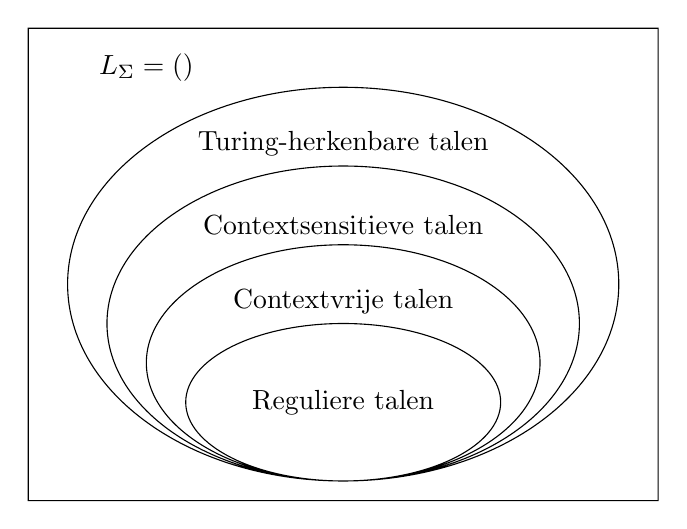
\begin{tikzpicture}
  \path
    (0,0) rectangle (8,6) [draw]
    (1.5,5.5) node {$L_\Sigma = \powerset(\sstar)$}
    (4,2.75) coordinate (A) node[above=1.5cm] {Turing-herkenbare talen} ellipse (3.5 and 2.5) [draw]
    (4,2.25) coordinate (B) node[above=1cm] {Contextsensitieve talen} ellipse (3 and 2) [draw]
    (4,1.75) coordinate (C) node[above=0.5cm] {Contextvrije talen} ellipse (2.5 and 1.5) [draw]
    (4,1.25) coordinate (D) node {Reguliere talen} ellipse (2 and 1) [draw];
\end{tikzpicture}
\end{center}

\textit{Zijn de talen van een TM beslisbaar?}

De verzameling van de talen die bepaald worden door een Turingmachine, of m.a.w. Turing-herkenbaar zijn is niet beslisbaar. Dit is equivalent met de vraag, kunnen we voor elke string $s \in L$ waarbij $L$ een taal is die door een machine $TM$ herkent wordt, beslissen dat $s$ door $TM$ geaccepteerd wordt? Dat is het acceptatieprobleem, wat niet beslisbaar is.

\subsection{Turingmachines}

\subsubsection{Vraag 1 - $\atm$}

\textit{Bewijs in detail dat $\atm$ niet beslisbaar is - steun daarbij niet op de stelling van Rice.}

We bewijzen dit door contradictie. Stel dat er een beslisser $B$ bestaat voor $\atm$. Bij een input $\langle M,s \rangle$ accepteert $B$ $M$ als $M$ $s$ accepteert en $B$ verwerpt $M$ als $M$ $S$ verwerpt of blijft lopen.

We construeren nu een contradictiemachine $C$ als
\begin{equation*}
C(\langle M \rangle) = opposite(B(\langle M,M \rangle))\text{ voor elke Turingmachine M}
\end{equation*}
De functie $opposite(x)$ is gedefinieerd als
\begin{equation*}
opposite(x) = \begin{cases}
reject, & \text{ als } x = accept\\
accept & \text{ als } x = reject
\end{cases}
\end{equation*}

We nemen nu $C(\langle C \rangle) = opposite(B(\langle C,C \rangle))$:
Als $C(\langle C \rangle) = accept$ ($C$ accepteert $C$), dan accepteert de beslisser $B$ de invoer $\langle C,C \rangle$, dus $B(\langle C,C \rangle) = accept$. Maar $opposite(B(\langle C,C \rangle))$ is dan $reject$, dat is een tegenstelling omdat dan geldt $C(\langle C \rangle) \neq opposite(B(\langle C,C \rangle))$.

We kunnen nu zeggen dat de machine $C$ niet kan bestaan, dus de beslisser $B$ kan ook niet bestaan. Bij gevolg is $\atm$ niet beslisbaar.

\textit{Zou het helpen als het toegelaten was op de stelling van Rice te steunen?}

Nee. We hebben de stelling van Rice bewezen door $\atm$ te reduceren naar $Pos_P$, om aan te tonen dat $Pos_P$ niet beslisbaar is omdat $\atm$ niet beslisbaar is. Met andere woorden, het bewijs voor de stelling van Rice steunt op het bewijs dat $\atm$ niet beslisbaar is en dus kan de stelling niet gebruikt worden om dat te bewijzen.

\textit{Is $\atm$ herkenbaar?}

Ja, $\atm$ is herkenbaar. We kunnen namelijk een enumerator machine bouwen dit $\atm$ herkent.

\textit{Is $\atm$ co-herkenbaar?}

Nee, indien het co-herkenbaar was, zou het ook beslisbaar moeten zijn omdat het herkenbaar is.

\subsubsection{Vraag 2 - $\etm$}

\textit{Geef het bewijs van de stelling $\etm$ is niet beslisbaar: doe dat zonder de stelling van Rice te gebruiken.}

  Stel dat $\etm$ beslisbaar is en $E$ is een beslisser voor $\etm$, dan kunnen we een beslisser $B$ voor $\atm$ construeren. Voor een gegeven invoer $\langle M,s \rangle$ construeren we een machine $M_s$ waarvoor geldt
  \begin{itemize}
  \item Gegeven een invoer $w$, als $w \neq s$, verwerpt $M_s$ de string $w$.
  \item Anders laat $M_s$ $M$ lopen op $w$ en geeft hetzelfde resultaat terug.
  \end{itemize}
  $M_s$ is een machine die enkel accept teruggeeft indien $M$ $s$ accepteert en anders reject. We laten $E$ lopen op $\langle M_s \rangle$:
  \begin{itemize}
  \item Als $E$ $M_s$ accepteert, dan laten we $B$ zijn input $\langle M,s \rangle$ verwerpen, omdat $M_s$ dan de lege taal bepaalt, wat enkel mogelijk is als $M$ $s$ verwerpt.
  \item Als $E$ $M_s$ verwerpt, dan laten we $B$ zijn input $\langle M,s \rangle$ accepteren, omdat $M_s$ dan niet de lege taal bepaalt, wat enkel mogelijk is als $M$ $s$ accepteert.
  \end{itemize}

\textit{Bespreek daarna de uitspraken $\etm$ is herkenbaar en $\etm$ is co-herkenbaar.}

Indien het herkenbaar was, zou het ook beslisbaar moeten zijn omdat het co-herkenbaar is.

$\etm$ is co-herkenbaar. We kunnen namelijk een enumerator machine bouwen dit $\overline{\etm}$ herkent.

\textit{Ken je ook alternatieve bewijzen?}

We kunnen dit bewijzen met de stelling van Rice. Bovendien is het ook mogelijk om aan te tonen dat $\etm$ beslisbaar is t.o.v. $\atm$ ($\etm \leq_T \atm$) met een orakel voor $\atm$:

  We construeren een Orakelmachine $\oatm$. Bij input $\langle M \rangle$ doet $\oatm$:
  \begin{itemize}
  \item Construeer een Turingmachine $P$ die bij input $w$:
  \begin{itemize}
  \item $M$ laat lopen op alle strings van $\sstar$.
  \item Als $M$ eender welke string van $\sstar$ accepteert, dan accepteert $P$ de input $w$. ($P$ accepteert voor eendere welke $w$ zo lang dat $M$ minstens \'e\'en string accepteert en dus niet de lege taal bepaalt.)
  \end{itemize}
  \item $\oatm$ vraagt aan het orakel of $\langle P,w \rangle \in \atm$.
  \item Als het orakel ``ja'' antwoordt, dan verwerpt $\oatm$ de invoer, omdat $M$ niet de lege taal bepaalt. Anders accepteert het de invoer.
  \end{itemize}
  
  $\oatm$ is een beslisser voor de taal $\etm$.

\textit{Hoe zit het met $E_{CFG}$?}

  We kunnen bewijzen dat $E_{CFG} = \{\langle G \rangle | G \text{ is een CFG en } L_G = \emptyset\}$ beslisbaar is door $G$ te transformeren als volgt:
  \begin{itemize}
  \item Voor een regel $A \rightarrow \alpha$ met $\alpha$ bestaande enkel uit terminals (inclusief $\epsilon$), dan:
  \begin{itemize}
  \item Verwijder alle producties waar $A$ aan de linkerkant staat.
  \item Vervang in elke regel waar $A$ rechts voorkomt, de voorkomens van $A$ door $\alpha$.
  \end{itemize}
  \item Herhaal de transformatie totdat:
  \begin{itemize}
  \item Het startsymbool verwijderd is, waarbij de invoer verworpen wordt, omdat dat betekent dat het mogelijk is een string af te leiden in het startsymbool.
  \item Er geen regels zijn van de benodigde vorm, waarbij de invoer aanvaard wordt, omdat de taal dan leeg is. (Het is dus niet mogelijk om een terminal te bereiken vanuit het startsymbool.)
  \end{itemize}
  \end{itemize}
  Door deze transformatie uit te voeren kunnen we voor elke CFG bepalen of die de lege taal bepaalt of niet en dus is $E_{CFG}$ beslisbaar.
  
  Merk op dat de grammatica getransformeerd wordt naar een niet-equivalente grammatica.

\subsubsection{Vraag 3 - Enumerator machine}

\textit{Definieer de enumerator machine.}

Een enumeratormachine is een variant van een Turingmachine (definitie \ref{def:tm}) met een extra enumeratortoestand $q_e$ en een overgangsfunctie met als signatuur \bm{$\delta: Q \times \Gamma \rightarrow Q \times \Gamma \times \Gamma_\epsilon \times \{L, R, S\}$}. Bij een overgang wordt voor $\Gamma_\epsilon$ in de signatuur een teken op een outputband geschreven. Bij het bereiken van $q_e$ wordt een outputmarker op de outputband geschreven die een outputstring afscheidt van de volgende.

\textit{Bewijs dat elke herkenbare taal kan ge\"enumereerd worden en dat elke taal die door een enumerator wordt ge\"enumereerd ook herkenbaar is.}

\paragraph{Elke herkenbare taal kan ge\"enumereerd worden.}
  Het Halting-probleem geeft aan dat een Turingmachine niet noodzakelijk stopt voor elke string. Daarom construeren we een enumerator $Enu$ voor een herkenbare taal $L$ bepaald door $TM$ als volgt:
 
  We construeren
  \begin{itemize}
  \item een Turingmachine $TM_{gen}$ die gegeven een getal $n$, de $n$ eerste strings van $\sstar$ op de band zet.
  \item een Turingmachine $TM_n$ die gegeven een getal $N$, op elk van de $n$ strings, $n$ stappen van $TM$ uitvoert. Als $TM$ daarbij een string accepteert, dan wordt die weggeschreven op de outputband van $Enu$.
  \item een Turingmachine $TM_{driver}$ die opeenvolgende getallen $n$ genereert en vervolgens $TM_{gen}$ en $TM_n$ oproept.
  \end{itemize}

\paragraph{Elke taal die door een enumerator wordt ge\"enumereerd is herkenbaar.}
We construeren een herkenner $H$ voor de taal $L$ bepaald door een gegeven enumerator $Enu$. Bij de invoer van een string $s \in L$ laat $H$ $Enu$ lopen. Telkens $Enu$ de toestand $q_e$ bereikt, vergelijkt $H$ de gegeven string $s$ met de laatste string op de outputband. Als ze gelijk zijn, dan accepteert $H$ de taal, als ze niet gelijk zijn, laat het $Enu$ de volgende string genereren.

\textit{Kan elke beslisbare taal ge\"enumereerd worden?}

Elke beslisbare taal is ook een herkenbare taal. Omdat elke herkenbare taal ge\"enumereerd kan worden kan ook elke beslisbare taal ge\"enumereerd worden.

\textit{Bespreek in deze context de uitspraak ``de verzameling van Turingmachines is een herkenbare taal''.}

Elke Turingmachine herkent een taal en elke herkenbare taal is enumereerbaar, dus moet ook de verzameling van alle Turingmachines enumereerbaar en dus herkenbaar zijn.

\subsubsection{Vraag 4 - Stelling van Rice}

\textit{Leg de stelling van Rice uit, en geef het bewijs.}

  Voor elke niet-triviale, taal-invariante eigenschap $P$ van Turingmachines geldt dat $Pos_P$ niet beslisbaar is. (Ook $Neg_P$ is niet beslisbaar, maar dat volgt uit $Neg_P = \overline{Pos_P}$.)

\paragraph{Bewijs.}   Stel dat $M_\emptyset$ die de lege taal bepaalt, een eigenschap $P$ niet heeft. Omdat $P$ niet-triviaal is, moet er een machine $X$ bestaat die de taal $L_X$ bepaalt en de eigenschap $P$ wel heeft.

  Stel dat er een beslisser $B$ bestaan voor $Pos_P$, dan kunnen we een beslisser $A$ voor $A_{TM}$ construeren. Voor een gegeven invoer $\langle M,s \rangle$ construeren we een hulpmachine $H_{M,s}$ waarvoor geldt
  \begin{itemize}
  \item $H_{M,s}$ laat $M$ lopen op $s$.
  \item Als $M$ $s$ accepteert, dan laat $H_{M,s}$ $X$ lopen op een invoer $x$ en accepteert indien $X$ $x$ accepteert.
  \end{itemize}
  
  We kunnen zeggen dat voor $H_{M,s}$ geldt dat het de taal $L_X$ bepaalt indien $M$ $s$ accepteert en de lege taal bepaalt indien $M$ $s$ niet accepteert. Dat wilt zeggen dat $H_{M,s}$ de eigenschap $P$ heeft indien $M$ $s$ accepteert en de eigenschap $P$ niet heeft indien $M$ $s$ niet accepteert.
  
  Bijgevolg kunnen we zeggen dat $A$ een invoer $\langle M,s \rangle$ accepteert als $B$ $H_{M,s}$ accepteert en de invoer verwerpt als $B$ $H_{M,s}$ verwerpt. Dus $A$ is een beslisser voor $\atm$, wat niet mogelijk is. Daarom kan de beslisser $B$ voor $Pos_P$ ook niet bestaan.
  
  We zeggen dat $\atm$ reduceerbaar is naar $Pos_P$.
  
  Als $M_\emptyset$ de eigenschap $P$ wel heeft, kunnen we het bewijs uitvoeren voor $\overline{P}$. Omdat we dan bewijzen dat $Pos_{\overline{P}} = Neg_P$ onbeslisbaar is, weten we dat ook $Pos_P = \overline{Neg_P}$ onbeslisbaar is.

\textit{Geef minstens \'e\'en eigenschap van Turingmachines die niet voldoet aan de voorwaarde voor de stelling van Rice, en laat zien dat die eigenschap geen aanleiding geeft tot een niet-beslisbare taal.}

De eigenschap ``de taal bepaald door een Turingmachine moet herkenbaar zijn'' is triviaal, omdat elke Turingmachine een Turing-herkenbare taal bepaalt. Dus deze eigenschap voldoet niet aan de stelling van Rice.

Indien deze eigenschap aanleiding zou geven tot een niet-beslisbare taal, dan zou elke herkenbare taal niet-beslisbaar moeten zijn. We weten echter dat elke beslisbare taal ook herkenbaar is.

\subsubsection{Vraag 4 (Bijvraag 1)}

\textit{Karakteriseer volledig alle eigenschappen van Turingmachines die aan de stelling van Rice voldoen m.b.v. $IsIn_{TM,S}$.}

$IsIn_{TM,S}$ is de verzameling van alle Turingmachines $M$ die een taal $L_M$ bepalen die deel uitmaakt van de verzameling $S$. We zoeken een eigenschap $P$ van een Turingmachine $M$ zodanig dat
\begin{equation*}
  L_M \in S \leftrightarrow M \in Pos_P \en M \notin Neg_P
\end{equation*} 

Indien de eigenschap $P$ aan de stelling van Rice voldoet, is $IsIn_{TM,S}$ niet beslisbaar, want dan geldt $IsIn_{TM,S} = Pos_P$.

\subsubsection{Vraag 5 - Orakelmachine}

\textit{Wat is een orakelmachine?}

Een orakelmachine is een Turingmachine die een orakel kan raadplegen om de oplossing voor een bepaald probleem te vragen.

Aan een orakel voor $\atm$ kan een TM bijvoorbeeld vragen of een machine $M$ een string $s$ accepteert.

\textit{Bespreek de uitspraak: "de verzameling orakelmachines (over een gegeven orakel) is strikt krachtiger dan de verzameling van Turing machines". Leg hierbij ook uit wat je bedoelt met "krachtiger".}

Een verzameling $A$ is krachtiger (of sterker) dan een verzameling $B$ indien $B$ een deelverzameling is van $A$.

De verzameling van orakelmachines over een gegeven orakel is krachtiger dan de verzameling van de Turingmachines, omdat een orakelmachine een Turingmachine is, dus voor elke Turingmachine bestaat een equivalente orakelmachine die het orakel niet raadpleegt. Bovendien kan een orakelmachine problemen beslissen die een Turingmachine niet kan beslissen, wat maakt dat de verzameling van orakelmachines groter is dan de verzameling van Turingmachines en dus krachtiger.

Een voorbeeld is de orakelmachine $\oatm$ met een orakel voor $\atm$, die in staat is om $\atm$ te beslissen en bij gevolg ook heel wat andere problemen.

\textit{Kan een verzameling orakelmachines (voor bepaald gegeven orakel) alle talen beslissen?}

Nee, de verzameling van orakelmachines is (oneindig) aftelbaar, maar de verzameling van alle talen $L_\Sigma$ is niet-aftelbaar. Daarom moet er minstens \'e\'n taal zijn die een orakelmachine voor een bepaald orakel niet kan beslissen.

\subsubsection{Vraag 5 (Bijvraag 1)}

\textit{Kan een orakelmachine voor $\atm$, $\htm$ beslissen?}

Ja, je kan een orakelmachine $\oatm$ construeren die voor een input $\langle M,s \rangle$ beslist of die machine stopt voor de string $s$. Dat gebeurt als volgt:

\begin{itemize}
\item De machine vraagt aan het orakel of $M$ $s$ accepteert. Indien het antwoord ``ja'' is, dan accepteert $\oatm$ de invoer.
\item Anders construeren we een machine $M_i$ die gelijk is een $M$ met de uitzondering dat de accepterende en verwerpende toestanden gewisseld zijn. De machine vraagt aan het orakel of $M_i$ $s$ accepteert. Indien het antwoord ``ja'' is, dan accepteert $\oatm$ de invoer.
\item Anders verwerpt $\oatm$ de invoer, omdat we dan weten dat $M$ niet zal stoppen.
\end{itemize}

We kunnen zeggen dat $\htm \leq_T \atm$. Bovendien, omdat we weten dat $\atm \leq_m \htm$ en dus ook $\atm \leq_T \htm$, zeggen we dat $\atm \equiv_T \htm$ ($\atm$ en $\htm$ zijn Turing-equivalent).

\subsubsection{Vraag 6 - Reduceerbaarheid}

\textit{Bespreek de twee noties van reduceerbaarheid ($A \leq_m B$ en $A \leq_T B$), hun verband en op welke manier die noties kunnen gebruikt worden om aan te tonen dat een taal (on)beslisbaar/herkenbaar is.}

\paragraph{Reduceerbaarheid.} Een taal $L_1$ over $\Sigma_1$ kan gereduceerd worden naar een taal $L_2$ over $\Sigma_2$ als er een afbeelding \bm{$f: \sstar_1 \rightarrow \sstar_2$} bestaat zodanig dat $f(L_1) \subseteq L_2$ en $f(\overline{L_1}) \subseteq \overline{L_2}$ met $f$ een Turing-berkenbare functie.

Indien een taal $A$ niet-beslisbaar is en reduceerbaar is naar een andere taal $B$, dan moet $B$ ook niet-beslisbaar zijn. Omdat we anders de beslisser van $B$ zouden kunnen gebruiken om $A$ te beslissen. We zeggen dus ook dat $A$ beslisbaar is als $B$ beslisbaar is. Dit geldt analoog voor herkenbaarheid.

\paragraph{Turingreduceerbaarheid.} Een taal $A$ is Turingeduceerbaar naar een taal $B$ indien er een orakelmachine $O^B$ bestaat die $A$ beslist. We zeggen dat $A$ beslisbaar is t.o.v. $B$.

Indien een taal $B$ beslisbaar is en een taal $A$ Turingreduceerbaar is naar $B$, dan moet $A$ ook beslisbaar zijn.

\paragraph{Verband.} Turingreduceerbaarheid is fijner dan reduceerbaarheid. Elk probleem $A$ dat reduceerbaar is naar $B$ moet ook Turingreduceerbaar zijn naar $B$.

\subsection{Lambda calculus}

\subsubsection{Vraag 1 - Church-Rosser}

\textit{Formuleer en bespreek de stellingen van Church-Rosser.}

\paragraph{CR1.}   Church-Rosser I verwijst naar de eerste stelling van Church en Rosser. Die stelling zegt dat indien $E_1 \stackrel{*}{\longleftrightarrow} E_2$ geldt, dat er een expressie $E$ moet bestaan in normaalvorm zodanig dat $E_1 \stackrel{*}{\longrightarrow} E$ en $E_2 \stackrel{*}{\longrightarrow} E$.

Uit de eerste stelling volgt de uniciteit van de normaalvorm. Dat wilt zeggen dat de normaalvorm van een expressie altijd uniek is en enkel kan verschillen onder $\alpha$-reductie.

\paragraph{CR2.}   Church-Rosser II verwijst naar de tweede stelling van Church en Rosser. Die stelling zegt dat indien $E \stackrel{*}{\longleftrightarrow} N$  bestaat met $N$ in normaalvorm, dat er een reductierij moet bestaan in normaalorde van $E$ naar $N$.

\textit{Geef daarbij hun belang i.v.m. het baseren van een programmeertaal op lambda-calculus.}

De eerste stelling is belangrijk omdat het in essentie zegt dat het reduceren van een lambda-expressie altijd hetzelfde resultaat zal produceren.

De tweede stelling is belangrijk omdat de reductie in normaalorde zorgt voor ``lazy evaluation''. Een techniek waarbij een expressie enkel wordt ge\"evalueerd indien de waarde van die expressie nodig is. Een voorbeeld daarvan is het evalueren van een ``OR'' expressie. Het tweede argument van die expressie zal enkel ge\"evalueerd worden indien het eerste argument naar ``FALSE'' evalueert, omdat anders het resultaat van de expressie reeds ``TRUE'' zal zijn.

\textit{Geef de relatie met de programmeertaal Haskell.}

$\lambda$-calculus vormt de basis van de klasse van functionele programmeertalen. Haskell is een voorbeeld van een functionele programmeertaal, vernoemd naar de wiskunde Haskell Curry, wiens achternaam ook gebruik wordt voor de techniek ``currying'' bij functionele (en logische) programmeertalen en wie ook \'e\'en van de meest gekende vastpuntcombinators heeft bedacht.

\subsubsection{Vraag 1 (Bijvraag 1)}

\textit{Is $\lambda$-calculus Turing-compleet?}

Ja, het is mogelijk om elke (universele) Turingmachine in $\lambda$-calculus voor te stellen, omdat het elke Turing-berkenbare functie kan voorstellen.

\subsubsection{Vraag 1 (Bijvraag 2)}

\textit{Hoeveel conversieregels ken je?}

Er zijn drie conversieregels, namelijk:

\begin{itemize}
\item $\alpha$-conversie: Het hernoemen van variabelen.
\item $\beta$-conversie: Functie evaluatie.
\item $\eta$-conversie: Equivalentie onder redundante $\lambda$-abstracties.
\end{itemize}

Een vierde conversieregel, $\delta$-conversie wordt meestal niet vermeld. Dat is de evaluatie van ingebouwde functies.

\subsubsection{Vraag 1 (Bijvraag 3)}

\textit{Laat daarna zien hoe je in zuivere lambda-calculus recursieve functies kan defini\"eren. Doe dat m.b.v. een voorbeeld recursieve functie verschillend van FAC uit de cursus.}

Het is mogelijk om in $\lambda$-calculus een recursieve functie gebruik te maken van een vastpuntcombinator. Dat is een zelf-replicerende expressie. De meest voorkomende vastpuntcombinator werd voorgesteld door Haskell Curry:
\begin{equation*}
  Y\ F = F\ (Y\ F) \text{ met } Y = \lambda f.\ (\lambda x.\ f\ (x\ x))\ (\lambda x.\ f\ (x\ x))
\end{equation*}

Stel dat een $\lambda$-calculus niet beschikt over een optel functie, maar wel over een functie $INC$ om een getal met \'e\'en te verhogen en $DEC$ om dat getal met \'e\'en te verlagen. We stellen een recursieve functie $PLUS$ op, die een getal bij een ander getal optelt.

\begin{equation*}
  H = \lambda f,a,b.\ (IF\ (=\ b\ 0)\ a\ (f\ (INC\ a)\ (DEC\ b))) \text{ met } PLUS = H\ PLUS
\end{equation*}

$H$ is het vastpunt voor $PLUS$, nu kunnen we de defini\"erende vergelijking $PLUS = H\ PLUS$ vervangen met de vastpuntcombinator, zodat we $PLUS = Y H$ bekomen.

We kunnen nu een bewerking met deze functie uitvoeren:

\begin{equation*}
\begin{aligned}
PLUS\ 4\ 1 = \\
Y\ H\ 4\ 1 = \\
H\ (Y\ H)\ 4\ 1 = \\
\lambda f,a,b.\ (IF\ (=\ b\ 0)\ a\ (f\ (INC\ a)\ (DEC\ b)))\ (Y\ H)\ 4\ 1 \longrightarrow \\
\lambda a,b.\ (IF\ (=\ b\ 0)\ a\ ((Y\ H)\ (INC\ a)\ (DEC\ b)))\ 4\ 1 \stackrel{*}{\longrightarrow} \\
(IF\ (=\ 1\ 0)\ 4\ ((Y\ H)\ (INC\ 4)\ (DEC\ 1))) \longrightarrow \\
(IF\ FALSE\ 4\ ((Y\ H)\ (INC\ 4)\ (DEC\ 1))) \longrightarrow \\
(Y\ H)\ (INC\ 4)\ (DEC\ 1) \stackrel{*}{\longrightarrow} \\
(Y\ H)\ 5\ 0 = \\
\lambda f,a,b.\ (IF\ (=\ b\ 0)\ a\ (f\ (INC\ a)\ (DEC\ b)))\ (Y\ H)\ 5\ 0 \longrightarrow \\
\lambda a,b.\ (IF\ (=\ b\ 0)\ a\ ((Y\ H)\ (INC\ a)\ (DEC\ b)))\ 5\ 0 \stackrel{*}{\longrightarrow} \\
(IF\ (=\ 0\ 0)\ 5\ ((Y\ H)\ (INC\ 5)\ (DEC\ 0))) \longrightarrow \\
(IF\ TRUE\ 5\ ((Y\ H)\ (INC\ 5)\ (DEC\ 0))) \longrightarrow \\
5
\end{aligned}
\end{equation*}